\section{Wahrnehmung}
\subsection{Wahrnehmungsprozess}
Kein passiv abbildender, sondern aktiver, konstruierender Vorgang!
\begin{enumerate}
	\item Distaler Stimulus
	\item Transformation Licht
		\begin{enumerate}
			\item Fokussieren auf Retina
			\item Proximaler Stimulus
		\end{enumerate}
	\item Sensorische Prozesse am Rezeptor
		\begin{enumerate}
			\item Transduktion
			\item Neuronale Repräsentation 
		\end{enumerate}
	\item Neuronale Verarbeitung
	\item Wahrnehmung
	\item Erkennen
	\item Handlen
\end{enumerate}
\subsection{Sehen}
\subsubsection{Physik}
Spezifische Wellenlängen (380 - 780 nm) werden als verschiedene Farben wahrgenommen.

\subsubsection{Fokussieren auf der Retina}
Cornea und Linse (80/20\% fix/variabel) fokussieren Bild auf Retina (Netzhaut). Visuelle Rezeptoren auf der Netzhaut (Stäbchen und Zapfen) enthalten visuelle Pigmente \rightarrow Transduktion. Sehnerv leitet Informationen von Retina ans Gehirn weiter.

\subsubsection{Transduktion im Visuellen Rezeptor}
Durch auftreffen von Licht auf den visuellen Rezeptor gehen die Na$^+$ Kanäle zu \Rightarrow Zelle wird hyperpolarisiert und schüttet weniger Glutamat aus

\subsubsection{Neuronale Verarbeitung}
\begin{center}
	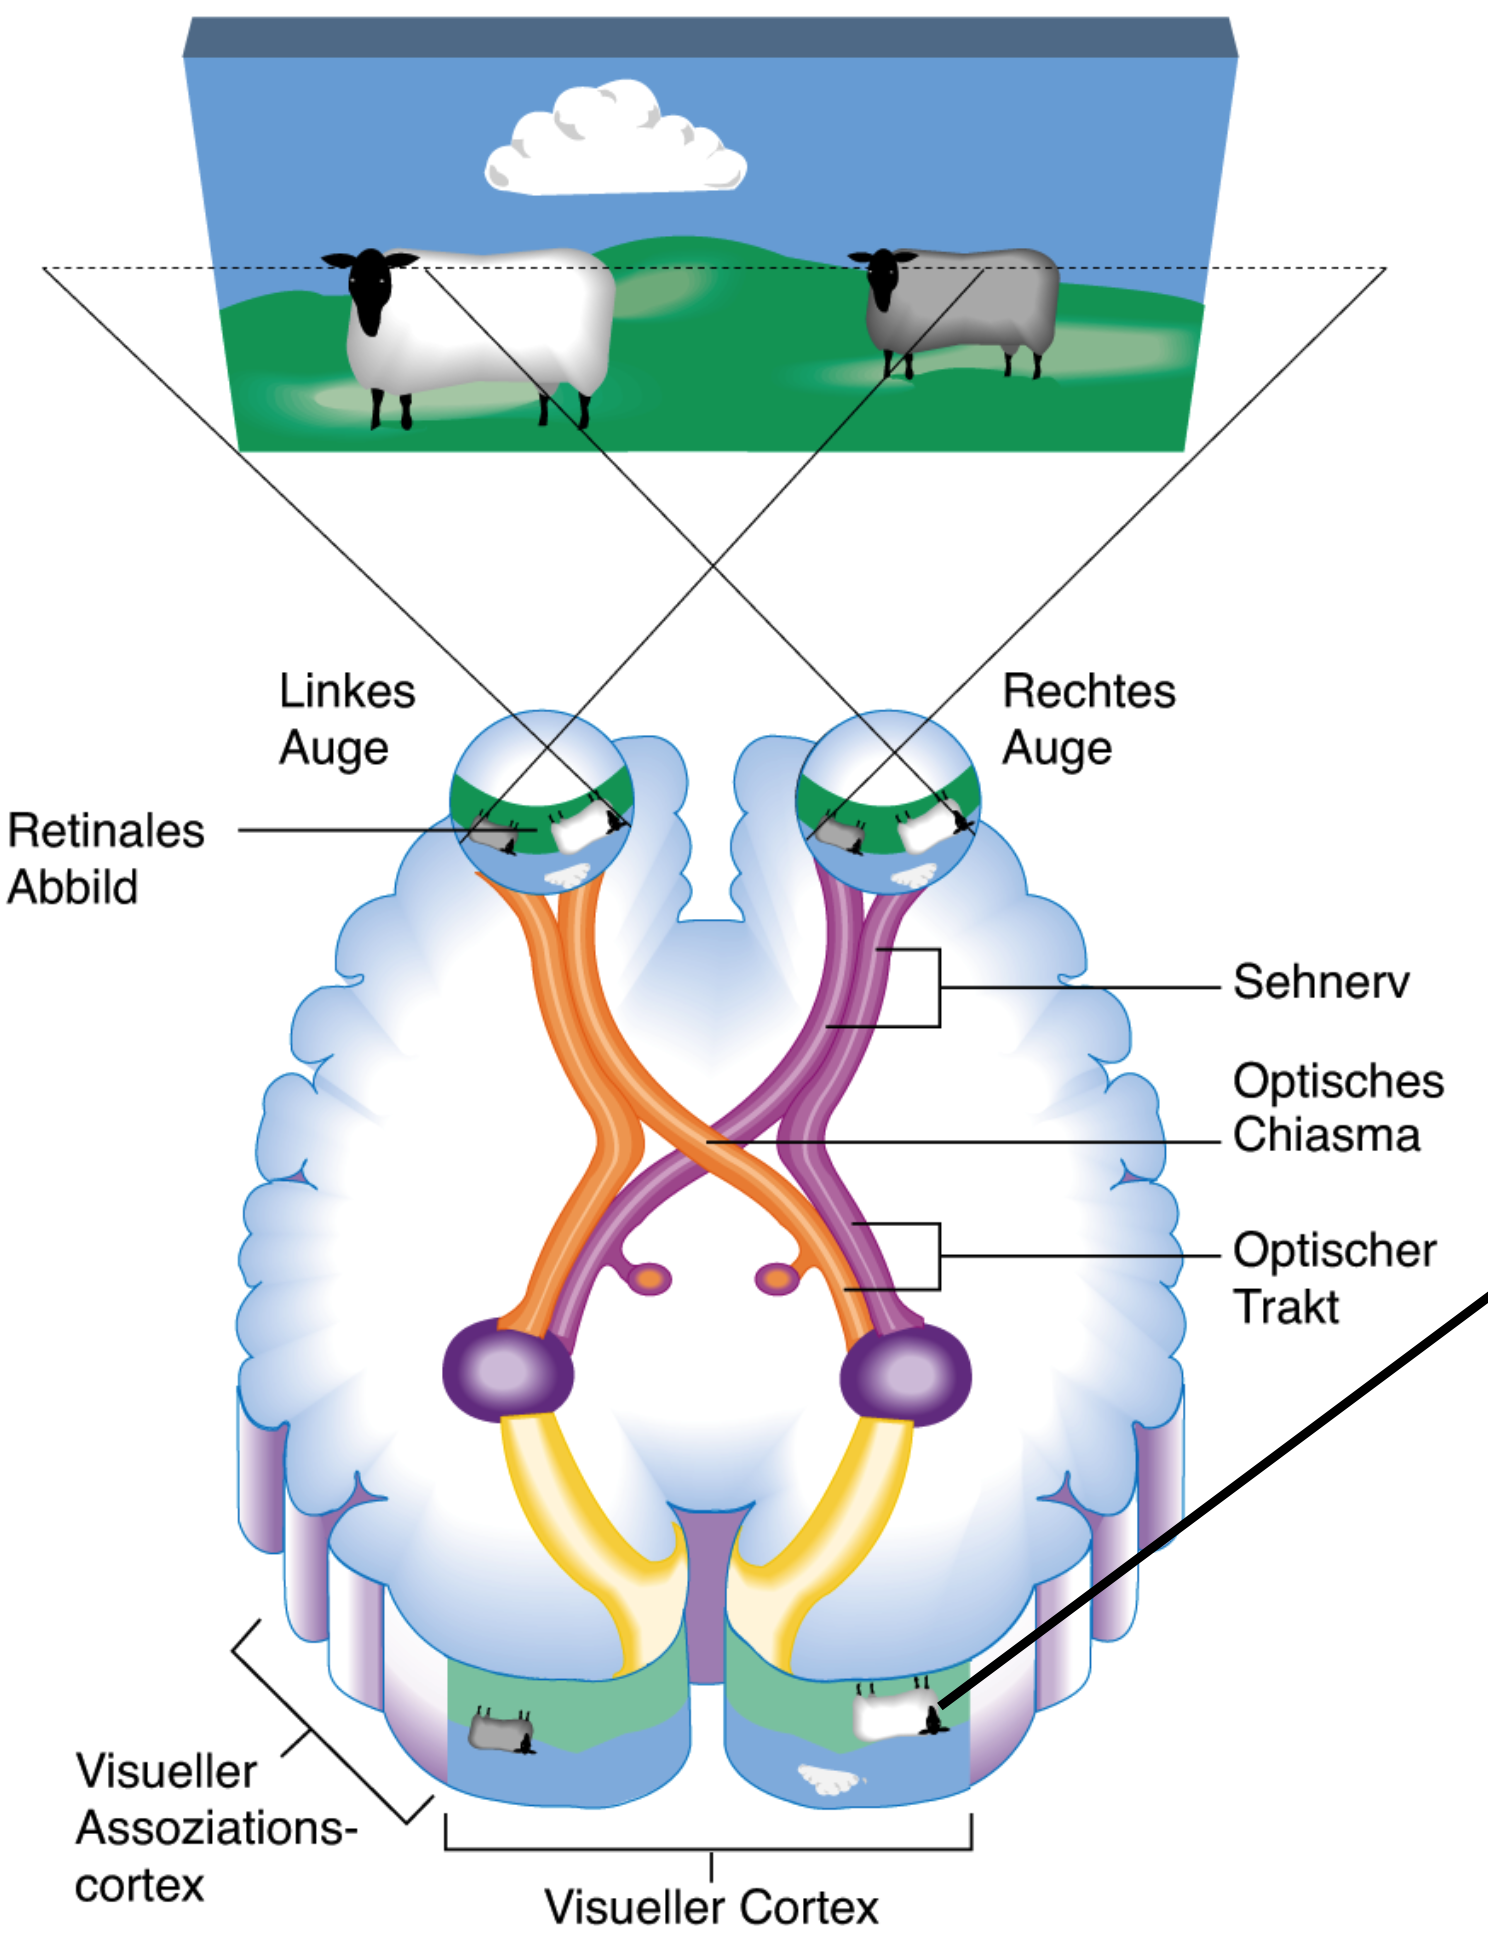
\includegraphics[scale=.2]{img/Auge.png}
\end{center}

\subsubsection{Verarbeitung Wellenlängen}
Zapfen:
\begin{itemize}
	\item S-Cone (Blau)
	\item M-Cone (Grün)
	\item L-Cone (Gelb)
\end{itemize}

\rightarrow Trichromatische Theorie

Gegenspieler-Verschaltung:
\begin{itemize}
	\item Rot-Grün (L-M)
	\item Blau-Gelb (S-(M+L))
	\item Schwarz-Weiß (S+M+L)
\end{itemize}

\rightarrow Gegenfarbtheorie
\subsection{Hören}
\subsubsection{Transformation \& Transduktion}
\begin{enumerate}
	\item Verstärkung des Frequenzbereichs der Sprache durch Resonanz
	\item Schwingung Luft \rightarrow Schwingung Flüssigkeit in Cochlea
	\item Schwingung der Basilarmembran verbiegt die Zilien der  Haarzellen \rightarrow Neurotransmitter-Ausschüttung 
\end{enumerate}
\subsubsection{Neuronale Repräsentation von Frequenzen}
Wie repräsentiert die Cochlea unterschiedliche Frequenzen des Schall?

Ortstheorie: Unterschiedliche Schallfrequenzen stimulieren unterschiedliche Orte und somit unterschiedliche Neuronenpopulationen der Basilarmembran optimal

\rightarrow Je stärker die Basilarmembran an einer Stelle schwingt, desto stärker freuen dorrt die Haarzellen 

\subsubsection{Neuronale Verarbeitung}
\begin{center}
	\includegraphics[scale=.2]{img/Ohr.png}
\end{center}

\subsubsection{Auditive Wahrnehmung}
\begin{itemize}
	\item Tonhöhe
		\begin{itemize}
			\item Perzeptuelle Unterscheidbarkeit von hohen vs. niedrigen Tönen aufgrund der Grundfrequenz des Tons (bis ca. 5000 Hz)
			\item Ganzzhaling Vielfache der Grundtonfrequenz hören sich ähnlich an und bilden eine Octave
		\end{itemize}
	\item Lautstärke
		\begin{itemize}
			\item Absolute Hörschwelle .0002 dB
		\end{itemize}
	\item Richtungshören durch drei Mechanismen
		\begin{itemize}
			\item Interaurale Laufzeitdifferenz
			\item Interaurale Pegeldifferenz
			\item Monoaurale spektrale Hinweisreize
		\end{itemize}
\end{itemize}










